\documentclass[a4paper,10pt]{extarticle}
\usepackage[T1]{fontenc}
\usepackage[utf8]{inputenc}
\usepackage{lmodern}
\usepackage{ngerman}
\usepackage[fleqn]{amsmath}
\usepackage{amssymb}
\usepackage{amsmath}
\usepackage{titlesec}
\usepackage{siunitx}
\usepackage{physics}
\usepackage{graphicx}
\usepackage{pdfpages}
\usepackage[T1]{fontenc}


\title{Übungsblatt 4}
\author{Lennard Behrens (3200335), Gabriel Kraus (3208414), Tizian Roth}

\begin{document}
\maketitle

\section{Aufgabe 1}
\subsection*{Aufgabe 1a}
Lässt man jegliche Reibungsfaktoren und die Ausbreitungsgeschwindigkeit des Signals außer acht, kann man den Steinwurf in den Brunnen als gleichmäßig beschleunigte Bewegungen ansehen, also
\begin{align*}
  a = \mbox{const} = g = 9,81 \mbox{m}/\mbox{s}^2 \mbox{.}
\end{align*}
Es wird angenommen, dass die Geschwindigkeit als auch die Beschleunigung parallel zu den Brunnenwänden ist. Daraus folgt für die Strecke abhängig von der Zeit
\begin{align*}
  s &= \frac{1}{2}\ddot{s}t^2\\
  s &= \frac{1}{2}gt^2 \mbox{.}
\end{align*}
Und umgekehrt gilt für die Fallzeit abhängig von der Strecke
\begin{align*}
  t = \sqrt{2\frac{s}{g}}
\end{align*}
Für die Tiefe bei $t=6\mbox{s}$ folgt dann
\begin{align*}
  s(6\mbox{s}) = 176.58\mbox{m}
\end{align*}
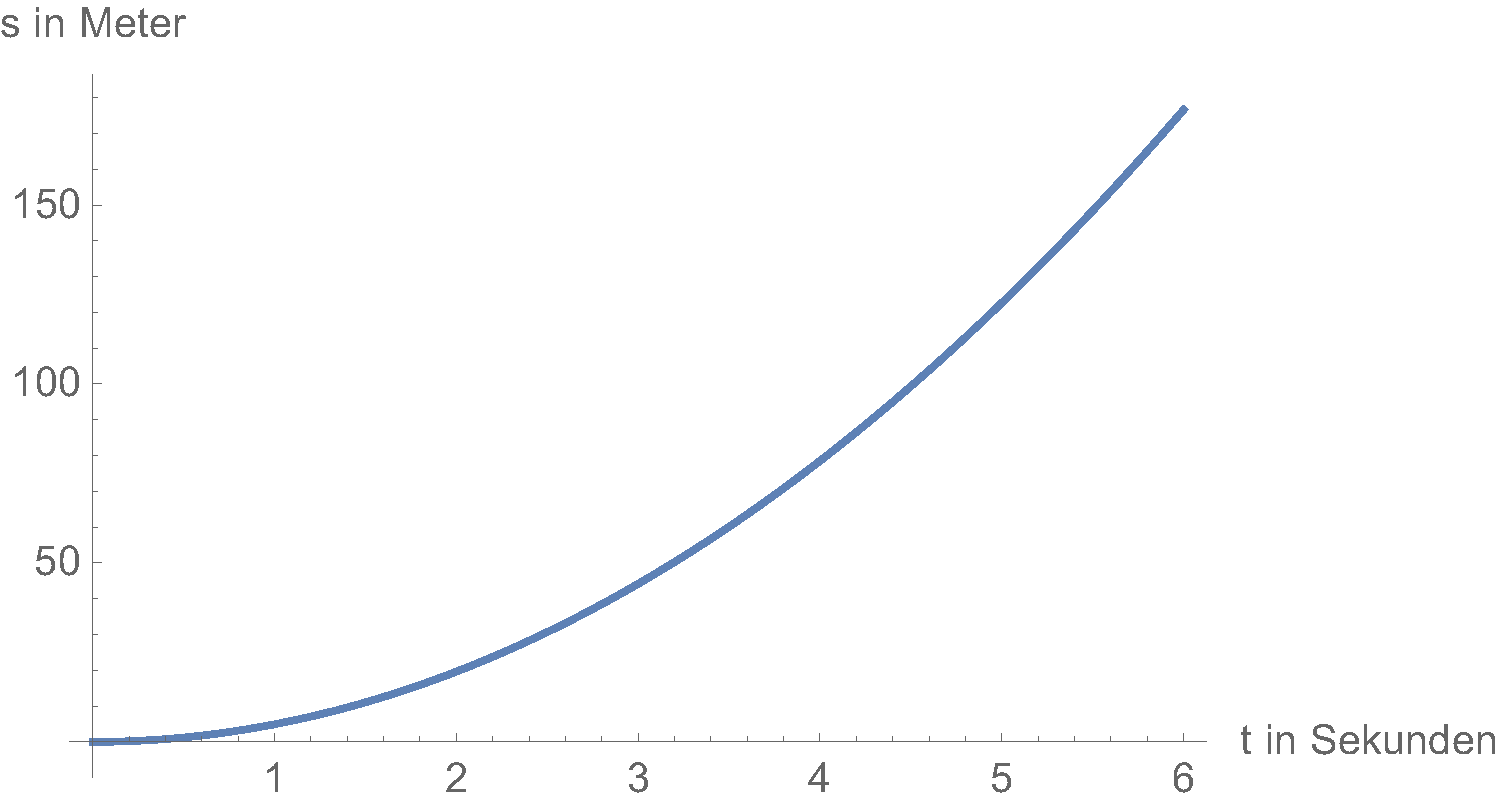
\includegraphics[scale=0.5]{./Abbildungen/Abbildung_01.pdf}
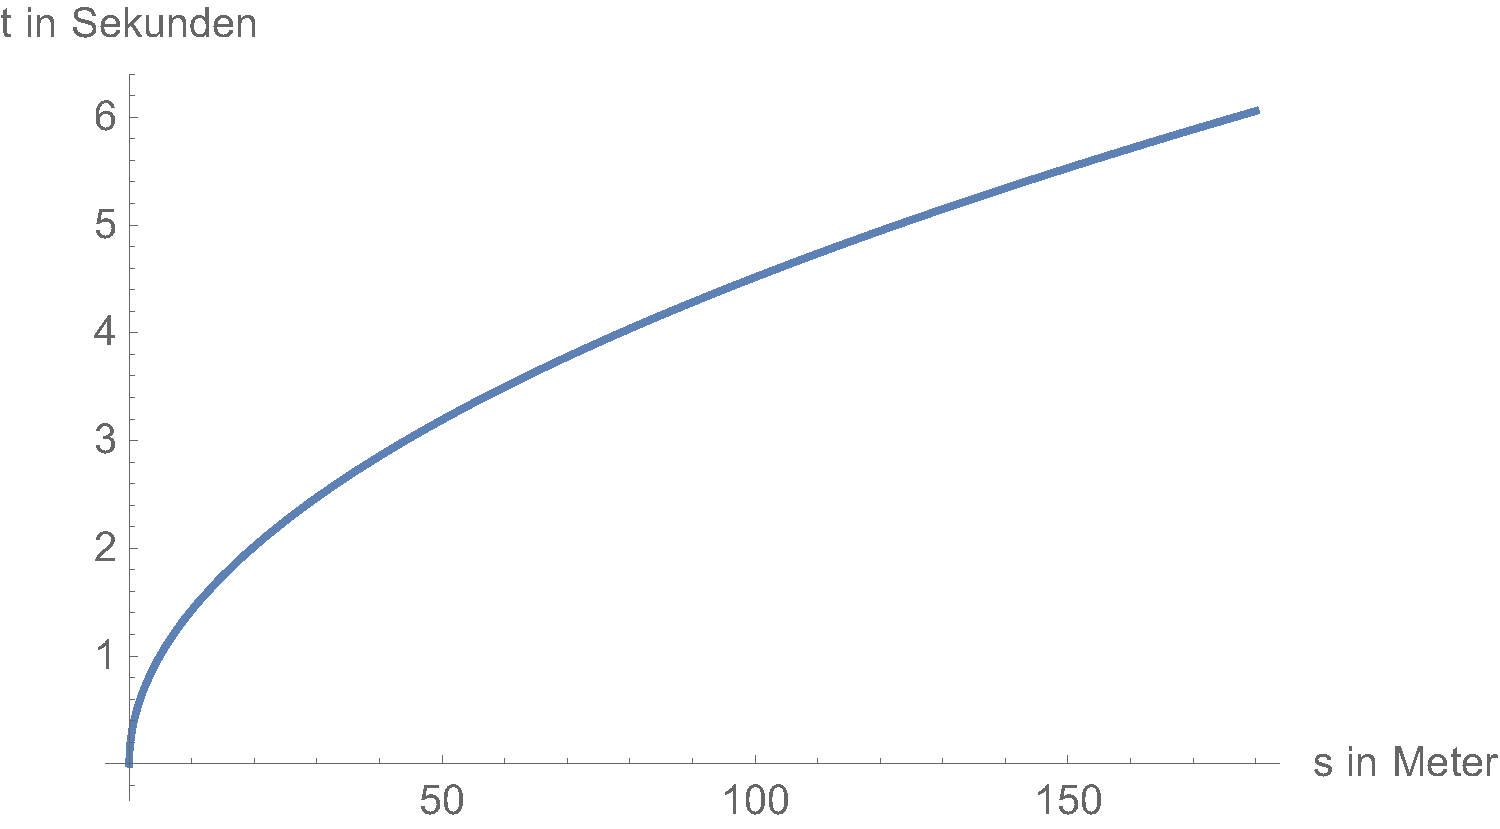
\includegraphics[scale=0.5]{./Abbildungen/Abbildung_02.pdf}

\subsection*{Aufgabe 1b}
Wenn man sowohl die Reibung als auch die Schallgeschwindigkeit berücksichtig, kann es zu erheblichen Abweichungen kommen. Da die Newton-Reibung proportional zum Quadrat der Geschwindigkeit ist, wird die Beschleunigung mit zunehmender Geschwindigkeit immer kleiner. Dies sorgt dafür, dass sich das fallende Objekt bei geeigneter Falltiefe einer Endgeschwindigkeit beliebig annähert. Für praktische Belange erreicht das Objekt nach einer gewisen Zeit eine Endgeschwindigkeit bzw die Beschleunigung ist nicht mehr konstant, sondern hat signifikant nachgelassen. Da sich das Geräusch des Aufschlags nur mit Schallgeschwindigkeit übertragen werden kann. wird mit zunehmender Tiefe und Geschwindigkeit des Objektes die Messung verfälscht. Man misst dann immer eine Falltiefe, die eigentlich zu groß ist. 
Das Kriterium für den Luftwiderstand ist bereits aus der Vorlesung bekannt. Hierfür wurde die Geschwindigkeit $v_E$ eingeführt. 
\begin{align*}
  v_E &= \sqrt{2\frac{mg}{c_w\rho A}}\\
  gt  &= \sqrt{2\frac{mg}{c_w\rho A}}\\
  t   &= \frac{1}{g}\sqrt{2\frac{mg}{c_w\rho A}}
\end{align*}
Spätestens ab dieser Fallzeit sollte man den Luftwiderstand aber auch die Schallgeschwindigkeit berücksichtigen, da dann die Beschleunigung näherungsweise null ist. 

\subsection*{Aufgabe 1c}
Die Zeit $t$ die gemessen wird, setzt sich nun aus der eigentlichen fallzeit $t_F$ und der Zeit, die das Geräusch zurück braucht $t_G$ zusammen.
\begin{align*}
  t &= t_F + t_G\\
  t &= \sqrt{2\frac{s}{g}} + \frac{s}{c} 
\end{align*}
Mithilfe der pq-Formel erhält man dann für $s(t)$ folgende Lösungen
\begin{align*}
  s_1 &= \frac{c^2}{g} + ct - \frac{\sqrt{c^4+2c^3gt}}{g}\\
  s_2 &= \frac{c^2}{g} + ct + \frac{\sqrt{c^4+2c^3gt}}{g}
\end{align*}
Im Sachzusammenhang macht jedoch nur 
\begin{align*}
  s_1 &= \frac{c^2}{g} + ct - \frac{\sqrt{c^4+2c^3gt}}{g}
\end{align*}
Sinn, da das eigentlich gemessene s kleiner wird. 
Für unser Messergebnis von $t = 6$s bedeutet das
\begin{align*}
  s(6\mbox{s}) = 151.35\mbox{m}
\end{align*}

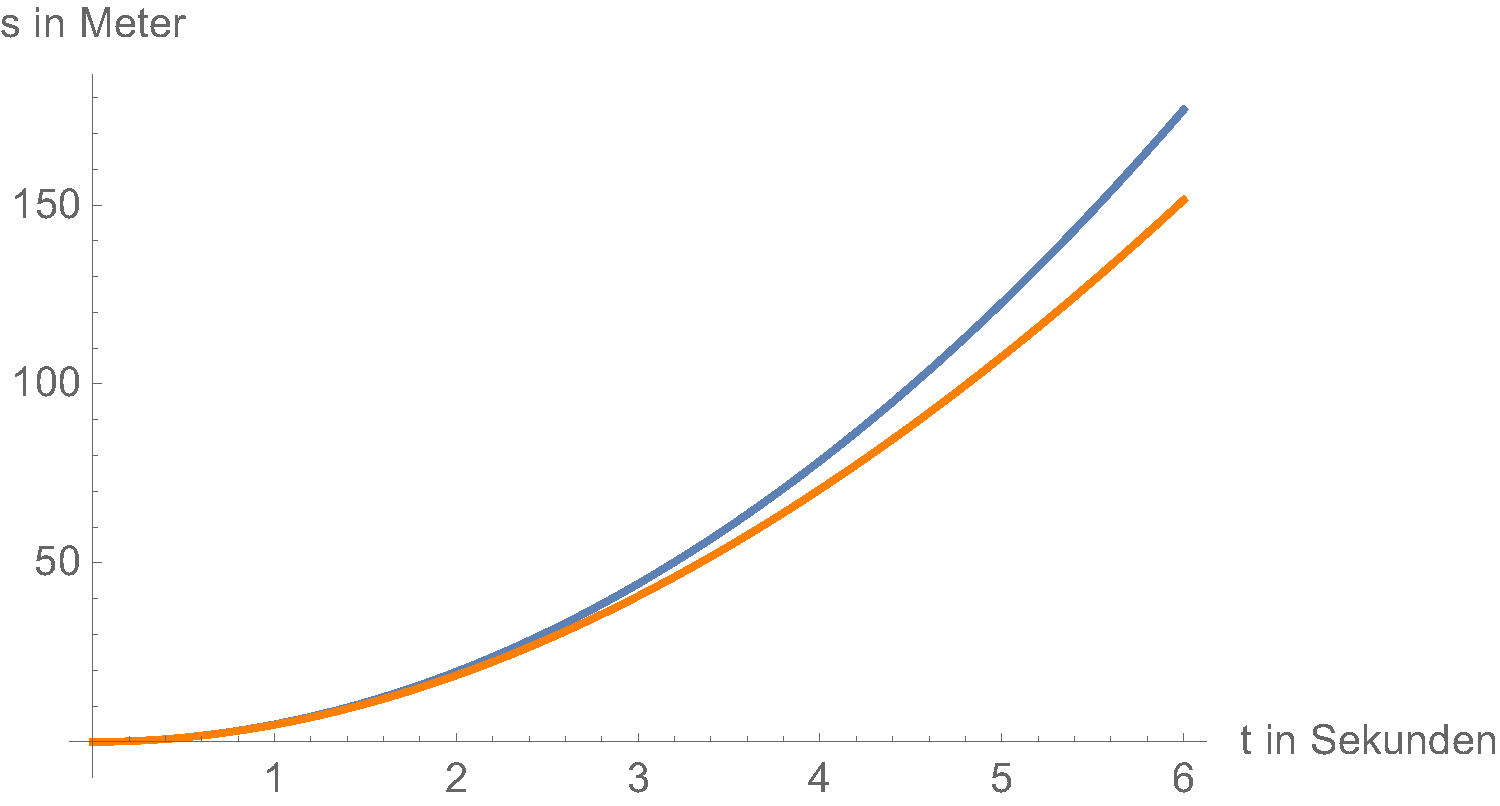
\includegraphics[scale=0.5]{./Abbildungen/Abbildung_03.pdf}
Hierbei ist die orangene Kurve diejenige, die die Schallgeschwindigkeit berücksichtigt.

\subsection*{Aufgabe 1d}
Für die Newtonreibung gilt
\begin{align*}
  F_R = \frac{1}{2}c_w\rho A v^2 \mbox{.}
\end{align*}
Aufgrund dieser Geschwindigkeitsabhängigen Reibung, ist die Beschleunigung ebenfalls nicht mehr konstant. 
Für das Kraft, die auf den Stein wirkt gilt dann
\begin{align*}
  m\ddot{s} &= m g - \frac{1}{2}c_w\rho A \dot{s}^2
\end{align*}
Wie in der Vorlesung besprochen ist die Lösung
\begin{align*}
  s   &= \frac{v_E^2}{g} \ln\left(\cosh\left(\frac{gt}{v_E}\right)\right)\\
  v_E &= \sqrt{2\frac{mg}{c_w\rho A}}
\end{align*}
Daraus folgt, dass 
\begin{align*}
  t  &= \frac{v_E}{g}\mbox{arcosh}(\exp(\frac{sg}{v_E^2}))
\end{align*}
Für die Masse des Steins gilt
\begin{align*}
  m = V_{Kugel} \rho_{stein} = \frac{4}{3}\pi r^3 \rho_{stein}
\end{align*}
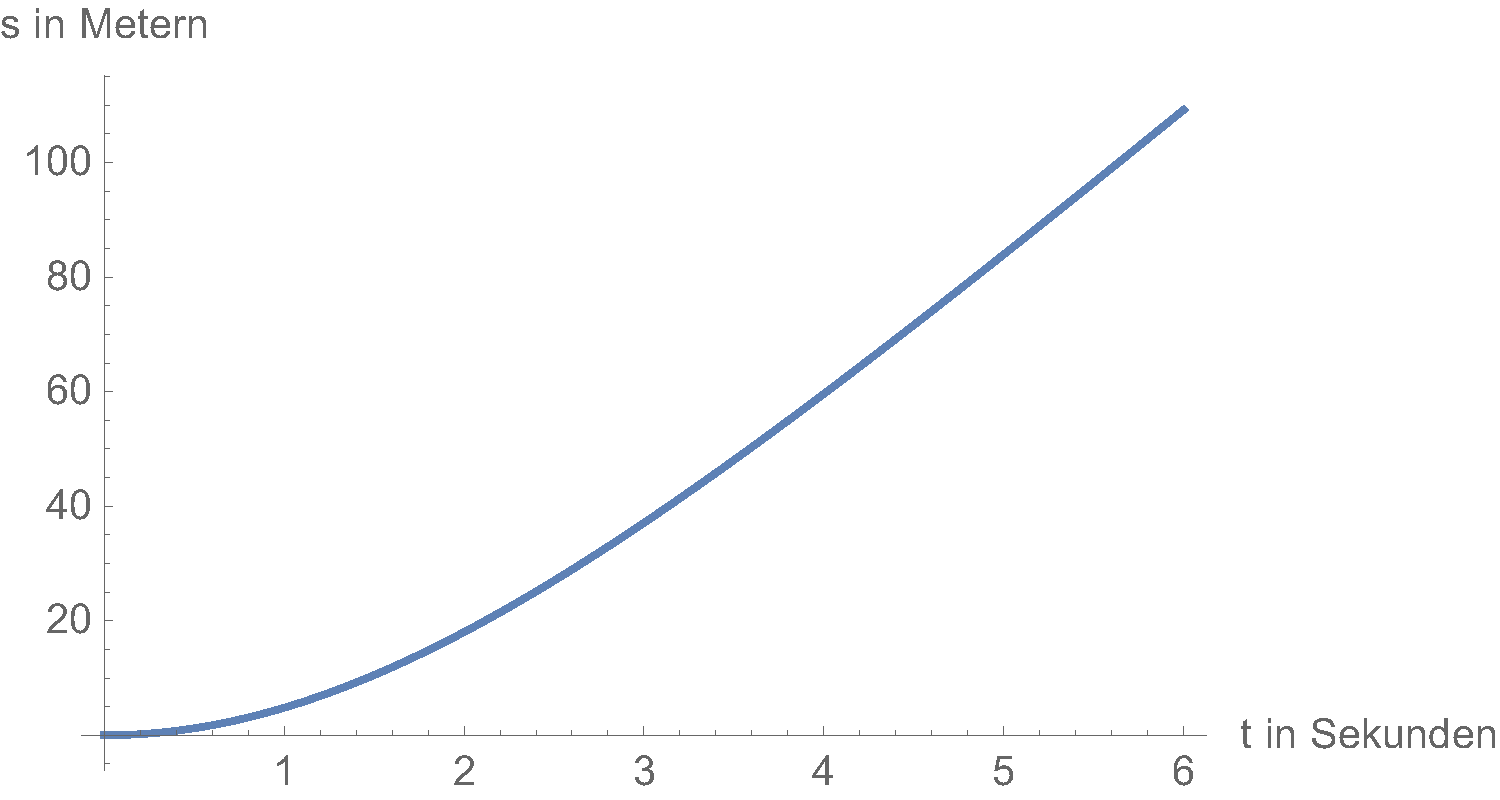
\includegraphics[scale=0.5]{./Abbildungen/Abbildung_04.pdf}
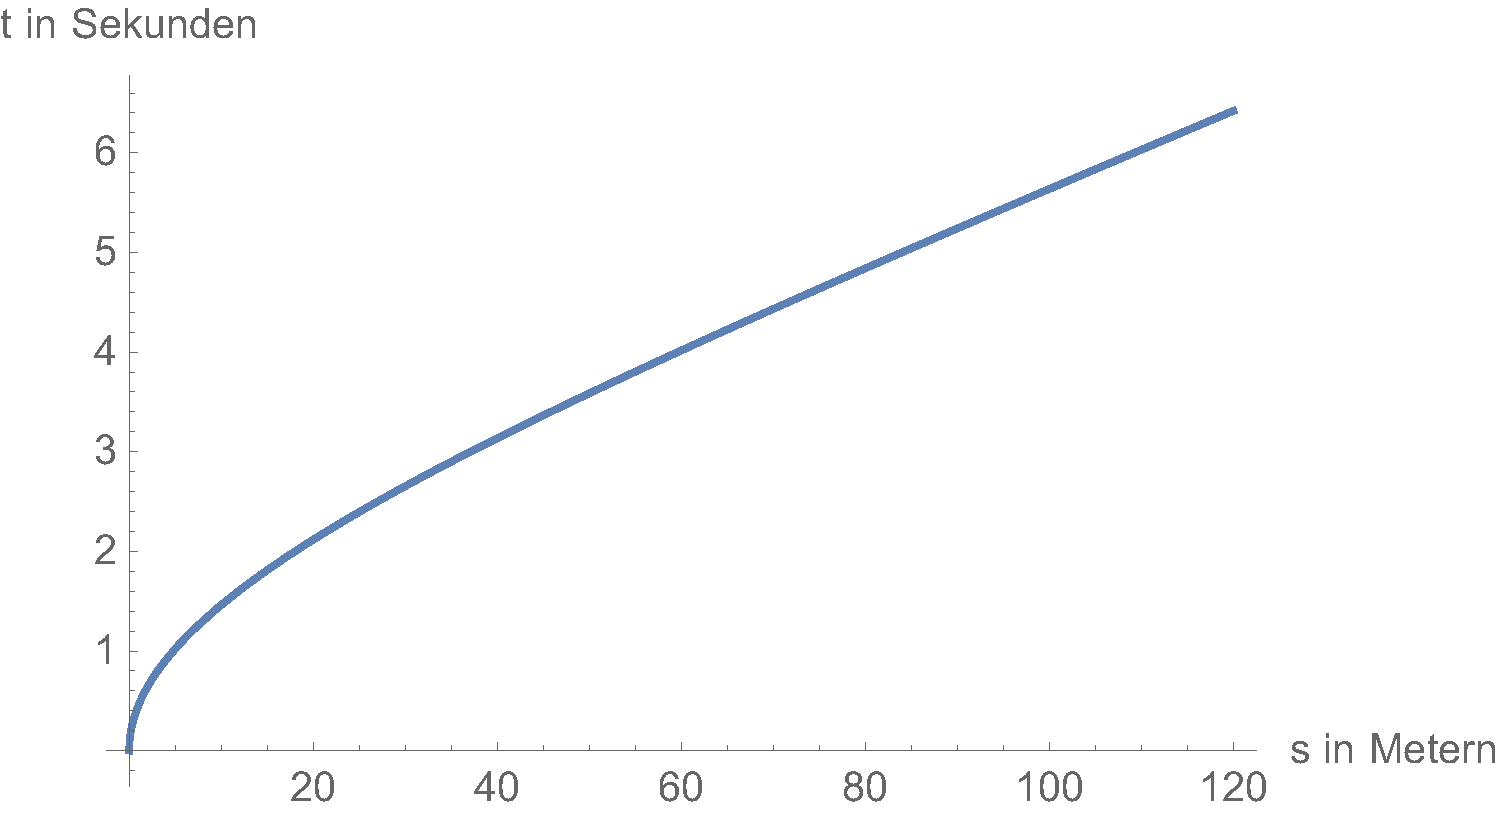
\includegraphics[scale=0.5]{./Abbildungen/Abbildung_05.pdf}

\subsection*{Aufgabe 1e}
Wenn man die Schallgeschwindigkeit berücksichtig kommt zu $t(s)$ aus Aufgabe 1d noch ein Term aus Aufgabe 1c dazu.
\begin{align*}
  t = \frac{v_E}{g}\mbox{arcosh}(\exp(\frac{sg}{v_E^2})) + \frac{s}{c}
\end{align*}
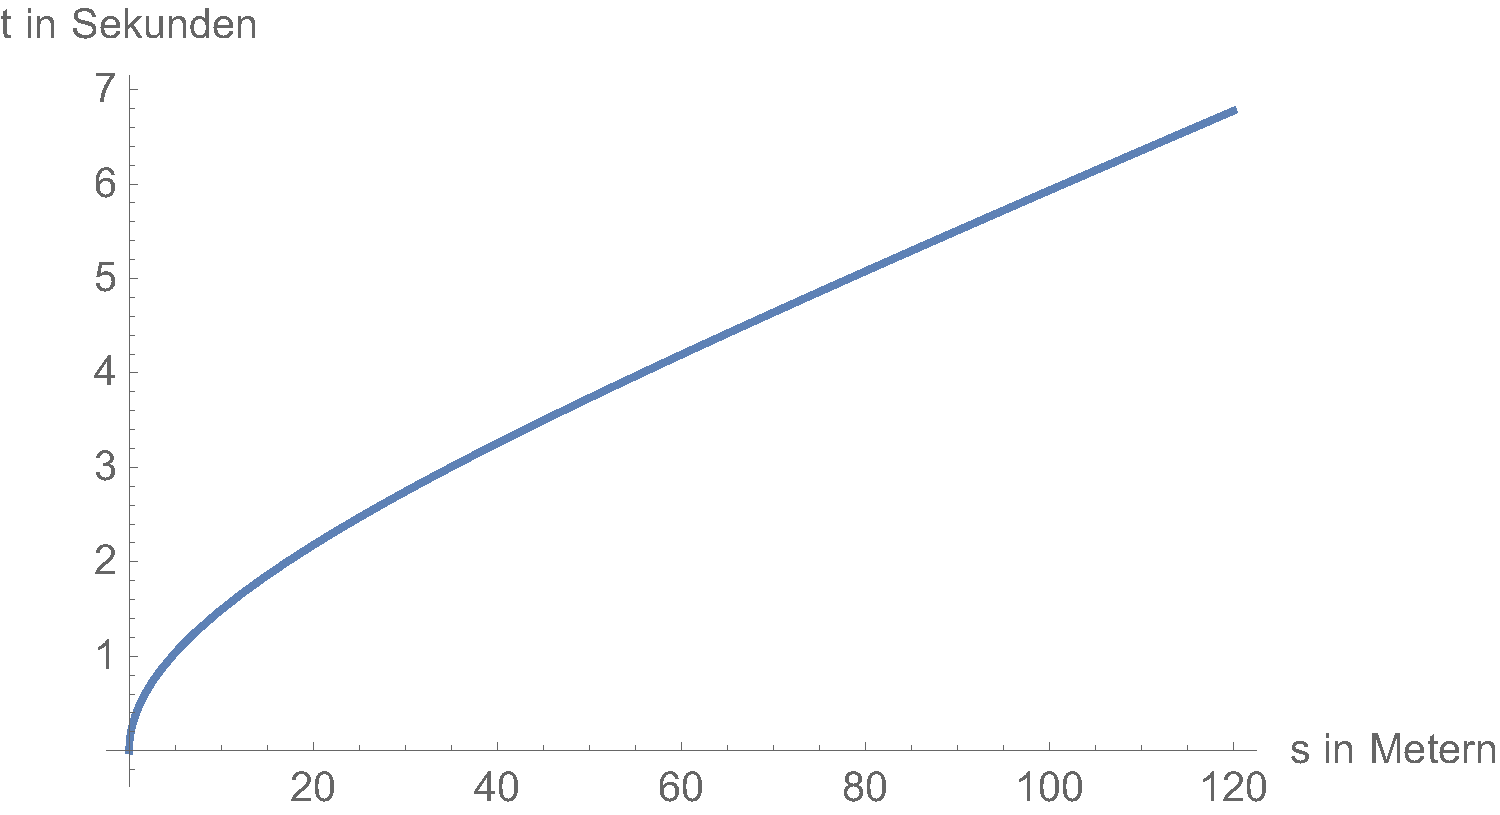
\includegraphics[scale=0.5]{./Abbildungen/Abbildung_06.pdf}
Nun kann man den Wert für s einfach ablesen:
\begin{align*}
  s \approx 100\mbox{m}
\end{align*}


\section*{Aufgabe 2}
\subsection*{Aufgabe 2a}
Ermittlung der Einheitsvektoren
\begin{align*}
x &= \cos(\varphi), \qquad y = \sin(\varphi), \qquad z = z \\
\varphi &= \omega t \\ \\
\pdv{\vec{r}}{\varrho} &= \cos(\omega t ) \hat{x} + \sin(\omega t ) \hat{y} \\ 
| \pdv{\vec{r}}{\varrho} | &= \sqrt{\cos(\omega t ) \hat{x} + \sin(\omega t ) \hat{y}} = 1 \\ 
\hat{\varrho}_{(t)} &= \frac{\pdv{\vec{r}}{\varrho}}{ | \pdv{\vec{r}}{\varrho} | } = \cos(\omega t ) \hat{x} + \sin(\omega t ) \hat{y} \\ \\
\pdv{\vec{r}}{\varphi} &= \varrho (-\sin(\omega t ) \hat{x} + \cos(\omega t ) \hat{y}) \\ 
| \pdv{\vec{r}}{\varphi} | &= \sqrt{\varrho (-\sin(\omega t ) \hat{x} + \cos(\omega t ) \hat{y})} = \varrho \\ 
\hat{\varphi}_{(t)} &= \frac{\pdv{\vec{r}}{\varphi}}{ | \pdv{\vec{r}}{\varphi} | } = -\sin(\omega t ) \hat{x} + \cos(\omega t ) \hat{y} \\ \\
\hat{z} &= \hat{z}
\end{align*}
Daraus ergeben sich die Zylinderkoordinaten: 
\begin{align*}
\vec{r_{(t)}} = \varrho_0 \hat{\varrho} + v_z t \hat{z}
\end{align*}

\subsection*{Aufgabe 2b}
$\vec{r}_{(t)}$ nach der Zeit ableiten.
\begin{align*}
\dot{\vec{r}}_{(t)} &= \varrho_0 \omega (-\sin(\omega t )\hat{x} + \cos(\omega t ) \hat{y}) + v_z \hat{z} \\
\dot{\vec{r}}_{(t)} &= \varrho_0 \omega \hat{\varphi} + v_z \hat{z} \\
\end{align*}

\subsection*{Aufgabe 2c}
$\dot{\vec{r}}_{(t)}$ nach der Zeit ableiten.
\begin{align*}
\ddot{\vec{r}}_{(t)} &= - \varrho_0 \omega^2 (\cos(\omega t )\hat{x} + \sin(\omega t ) \hat{y}) \\
\ddot{\vec{r}}_{(t)} &= - \varrho_0 \omega^2 \hat{\varrho} \\
\end{align*}


\section*{Aufgabe 3}
\subsection*{Aufgabe 3a}
Für kleine Winkel verhält sich der Sinus annähernd linear. Deshalb kann man auch die Kleinwinkelnäherung anwenden. Der Sinus flacht mit steigendem Winkel jedoch ab und verhält sich nichtmehr lienar. Mit der Kleinwinkelnäherung überschätzt man die Rückstellkraft bei größeren Winkeln stark. Gegeben sei die tatsächliche Rückstellkraft $F_R$ und die anngenäherte Rückstellkraft $F_N$. Daraus folgt für den Faktor $k$:
\begin{align*}
  F_R &= k\cdot F_N\\
  k   &= F_R / F_N = \frac{\sin\varphi}{\varphi}\\
  k\left(\frac{\pi}{2}\right) &= \frac{2}{\pi}
\end{align*} 
\subsection*{Aufgabe 3b}
Nachfolgend wird das Mathematica Notebook eingefügt. Man erkennt, ganz klar, dass sich die Näherung für kleine Anfangswinkel fast genau so verhält, wie die tatsächliche Lösung.
 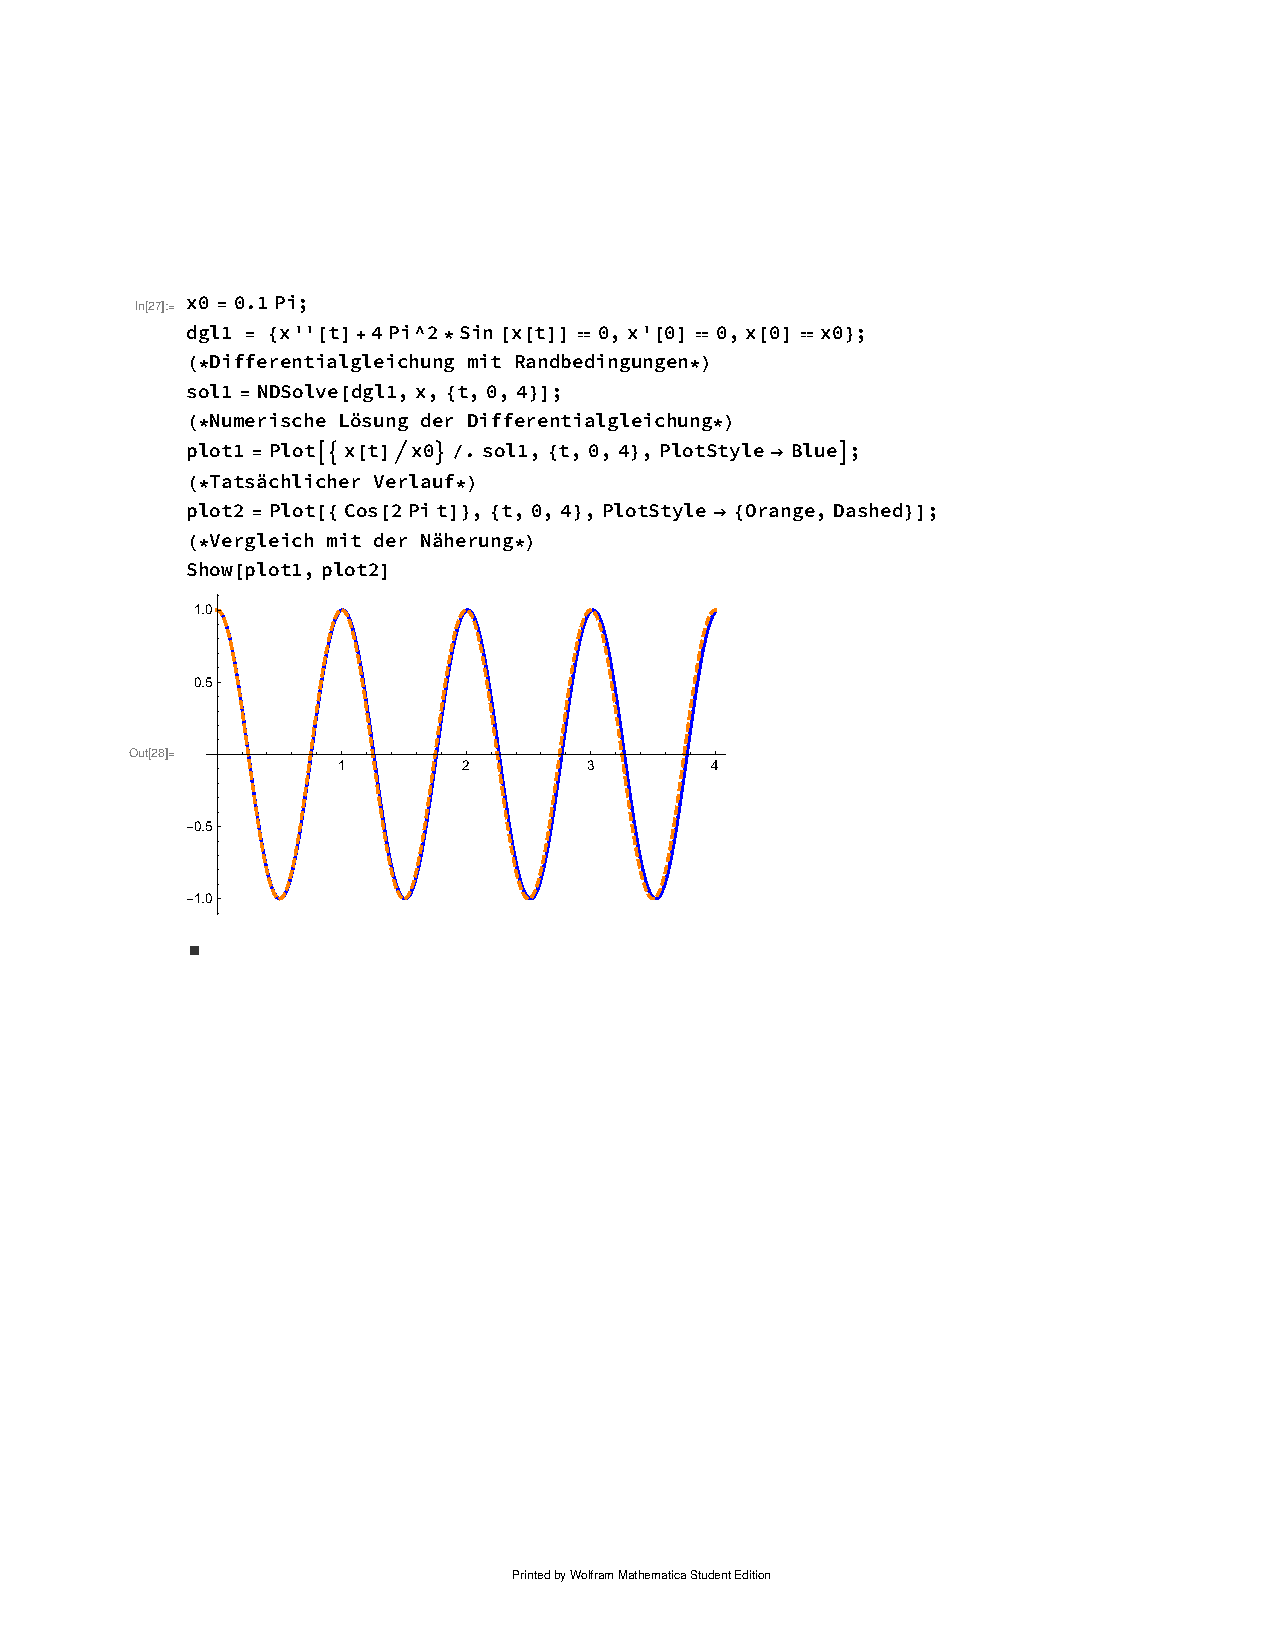
\includepdf[pages=-]{./Abbildungen/Abbildung_07.pdf} 
%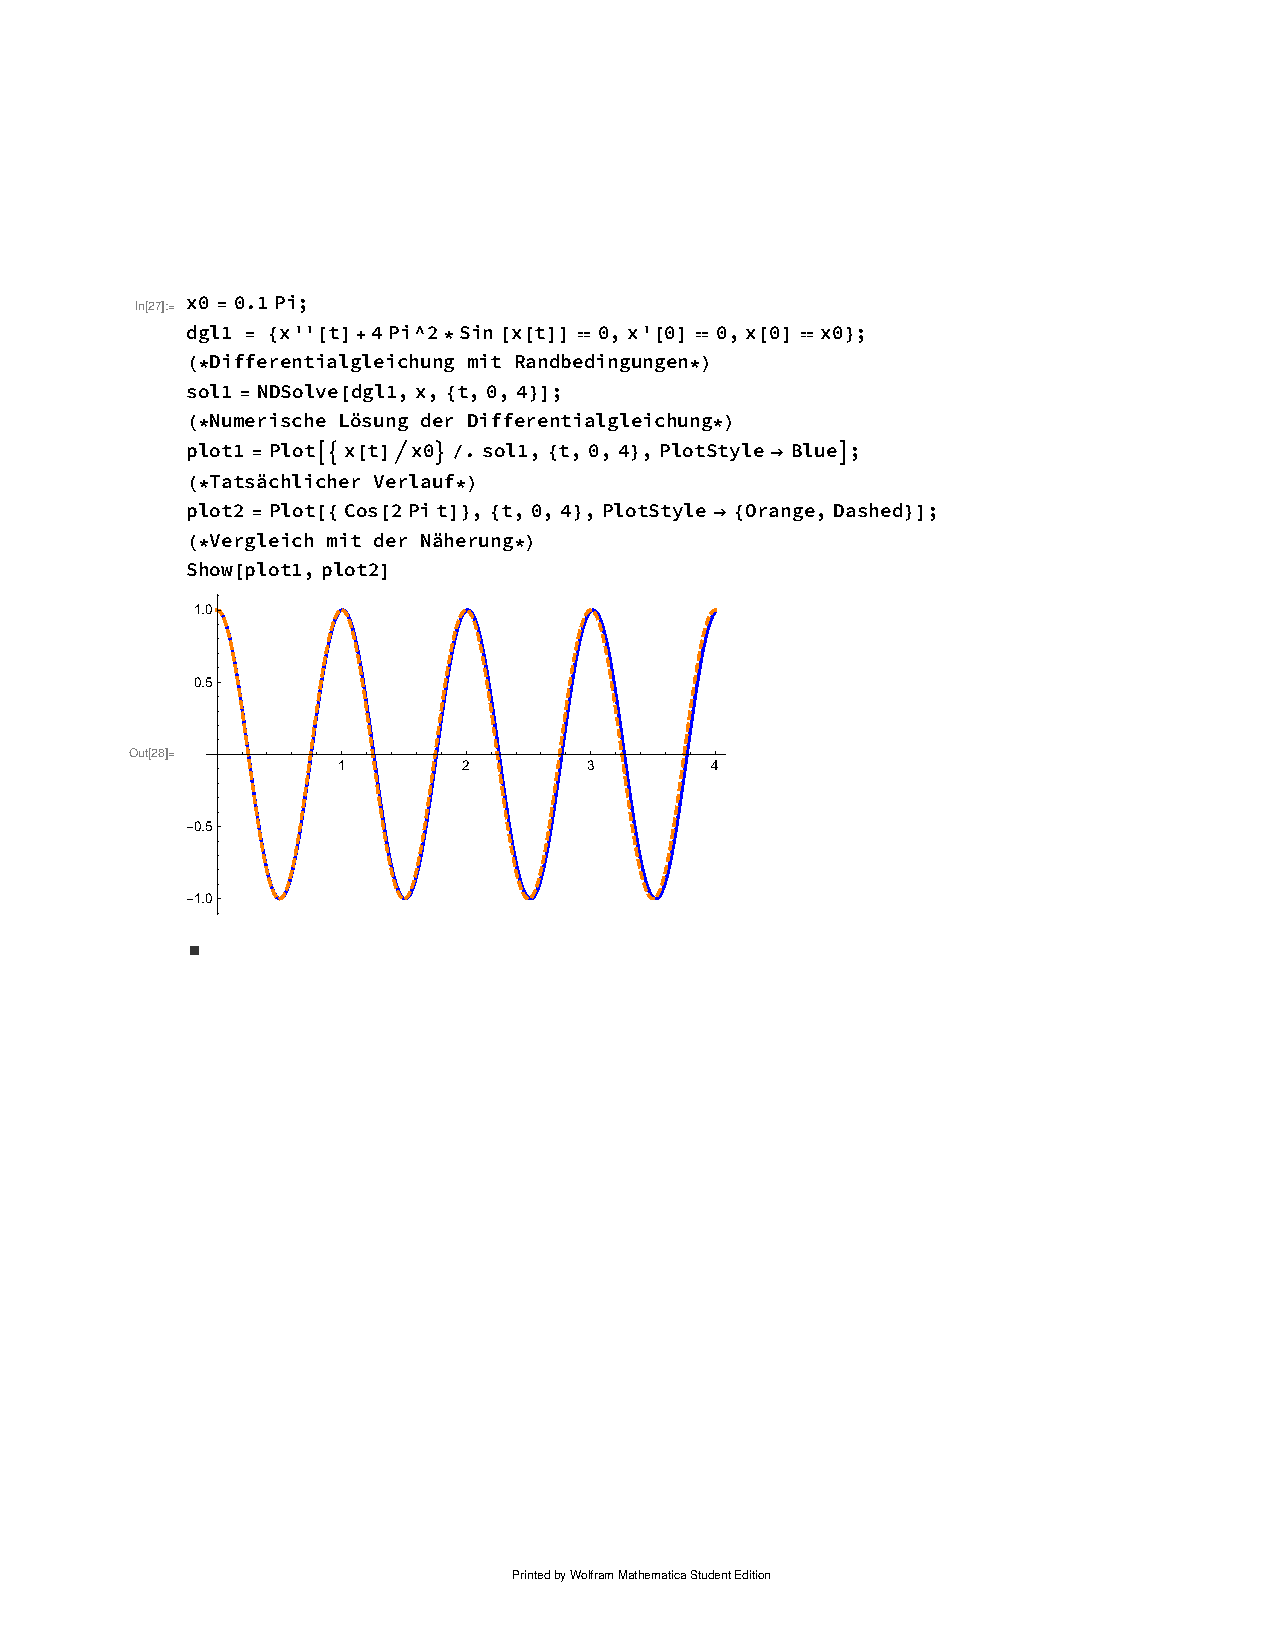
\includegraphics[scale=0.5]{./Abbildungen/Abbildung_07.pdf}


\section*{Aufgabe 4}
  \subsection*{Aufgbe 4a}
  Für die Übersicht wird $\pdv{x}{q_1}$ als $a$, $\pdv{x}{q_2}$ als $b$, etc. dargestellt.
  \begin{align*}
  \det \left(\begin{array}{c c c}
    a & b & c \\
    d & e & f \\
    g & h & i \\
  \end{array}\right) &= a \begin{vmatrix} e & f \\ h & i \end{vmatrix} - b \begin{vmatrix} d & f \\ g & i \end{vmatrix} + c \begin{vmatrix} d & e \\ g & h\end{vmatrix} \\
  &= aei - ahf - bdi + bgf + cdh - cge \\ \\
  \begin{pmatrix} a \\ d \\ g \end{pmatrix} \cdot \begin{pmatrix} \begin{pmatrix} b \\ e \\ h \end{pmatrix} \times \begin{pmatrix} c \\ f \\ i \end{pmatrix} \end{pmatrix} &= \begin{pmatrix} a \\ d \\ g \end{pmatrix} \cdot \begin{pmatrix} ei - hf \\ hc - bi \\ bf - ec \end{pmatrix} \\
  &= aei - ahf + dhc - dbi + gbf - gec
  \end{align*}
  Die beiden Ausdrücke sind gleich, was zu zeigen war.

  \subsection*{Aufgabe 4b}
  Volumenelement in Zylinderkoordinaten:
  \begin{align*}
  D &= \det \left(\begin{array}{c c c}
    \pdv{x}{\varrho} & \pdv{x}{\varphi} & \pdv{x}{z} \\
    \pdv{y}{\varrho} & \pdv{y}{\varphi} & \pdv{y}{z} \\
    \pdv{z}{\varrho} & \pdv{z}{\varphi} & \pdv{z}{z} \\
  \end{array}\right) \\
  &= \det \left(\begin{array}{c c c}
    \cos(\varphi) & -\varphi \sin(\varphi) & 0 \\
    \sin(\varphi) & \varrho \cos(\varphi) & 0 \\
    0 & 0 & 1 \\
  \end{array}\right) \\
  &= \varrho \cos^2(\varphi) + \varrho \sin^2(\varphi) = \varrho \\ \\
  dD &= \varrho \,d\varrho \, d\varphi \, dz
  \end{align*}

  Volumenelement in Kugelkoordinaten:
  \begin{align*}
  D &= \det \left(\begin{array}{c c c}
    \pdv{x}{\varrho} & \pdv{x}{\theta} & \pdv{x}{\varphi} \\
    \pdv{y}{\varrho} & \pdv{y}{\theta} & \pdv{y}{\varphi} \\
    \pdv{z}{\varrho} & \pdv{z}{\theta} & \pdv{z}{\varphi} \\
  \end{array}\right) \\
  &= \det \left(\begin{array}{c c c}
    \sin(\theta)\cos(\varphi) & \varrho \cos(\theta) \cos(\varphi) & - \varrho \sin(\theta) \sin(\varphi) \\
    \sin(\theta) \sin(\varphi) & \varrho \cos(\theta) \sin(\varphi) & \varrho \sin(\theta) \cos(\varphi) \\
    \cos(\theta) & - \varrho \sin(\theta) & 0 \\
  \end{array}\right) \\
  &= \sin(\theta) \cos(\varphi) (- \varrho^2 \sin^2(\theta) \cos(\varphi)) \\
  & \quad - \varrho \cos(\theta) \cos(\varphi) (\varrho \cos(\theta) \sin(\theta) \cos(\varphi)) \\ 
  & \quad - \varrho^2 \sin(\theta) \sin^2(\varphi) \\
  &= - \varrho^2 \left(\sin^3(\theta) \cos^2(\varphi) + \sin(\theta) \cos^2(\theta) \cos^2(\varphi) + \sin(\theta) \sin^2(\varphi)\right) \\ 
  &= - \varrho^2 \sin(\theta) \left( \sin^2(\theta) \cos^2(\varphi) + \cos^2(\theta) \cos^2(\varphi) + \sin^2(\varphi) \right) \\
  &= - \varrho^2 \sin(\theta) \left( \cos^2(\varphi) + \sin^2(\varphi) \right) \\
  &= - \varrho^2 \sin(\theta) \\
  &\mbox{Da man im Volumenelement den Betrag nimmt, folgt} \\ \\
  dD &= r^2 \sin(\theta) \,d\varrho \, d\varphi \, dz
  \end{align*}
\end{document}
